  \subsection{Emergency}


\begin{table}[H]
	\centering
    
    \begin{tabular}{|p{3.5cm}|p{10.3cm}|}
    
    \hline
    \textbf{\large{Actors}}  			& User 									\\
    				 					
    \hline
    \textbf{\large{Goals}} 				& \ref{goal:user0};\ref{goal:user00}\\
    
    \hline
    \textbf{\large{Enter Condition}}	& There is no enter condition for this Use Case		\\
    
    \hline
    \textbf{\large{Events Flow}}		& \begin{enumerate}[leftmargin=0.5cm]
                                          	\item The \emph{Visitor}  accesses to the web site or application log in page
                                            \item The \emph{Visitor} inserts all the mandatory informations (personal data, password, email)
                                            \item The System registers the user and sends back a confirmation email to the provided address
                                            \item The \emph{Visitor} user becomes a \emph{Registered user} inserting their fiscal code (if is a normal user) or the unique username (if is a third part), and the password in the log in page   
                                            \item The \emph{Registered user} now can access the \emph{TrackMe} services through the log in page
                                            
                                            \item After the insertion of the identifier and password, the user becomes a \emph{Logged in user}
                                          \end{enumerate}
    										\\
    \hline
    \textbf{\large{Exit Condition}} 	& The user is registered in the \emph{TrackMe} System, and his account is added to they system. Now the users is able to use all the functionalities provided by the system. \\
    
    \hline
    \textbf{\large{Exception}} 			& The \emph{Visitor} cannot register himself because is already registered.\newline The \emph{Registered} user                                         is not able to sign in the System because the login data are wrong or if he did not confirmed  the confirmation email. \newline
    								
    
    \hline
    
    
    \end{tabular}
	
\end{table}
\begin{figure}[H]
    \centering
    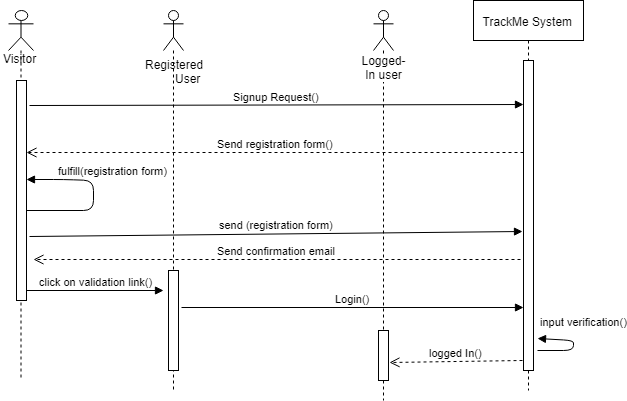
\includegraphics[scale=0.4]{rasdL/Pictures/login1.png}
    
\end{figure}
